\documentclass{article}

\usepackage[margin=1in]{geometry}
\usepackage{graphicx} 
\usepackage{gensymb}
\usepackage{amsmath}
\usepackage{multicol}
\usepackage{hyperref}
\usepackage[font=small,labelfont=bf]{caption}

\title{Filter}

\begin{document}

\begin{center}
    {\huge{How the Scalar function works}}
\end{center}    
    \begin{multicols}{2}
    The main problem of the data generated by the model is the scale of the data itself.
    As we can see in the following picture, the serie seems realistic if we just look at the trend.
    However, the magnitude of the data is totally out of scale. The algorithm below is designed to force
    the series to converge to the real data range.
    \subsection*{Introduction}
    The scaler aims at scaling the time serie without affecting the trend. The idea is that when we have 
    a peak of returns in the time serie, the significance of the peak depends on its distance from the second highest peak in the serie. For exemple let's take the following series from the dataset of stock values:\\
    \begin{center}
        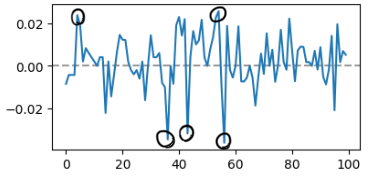
\includegraphics[scale = 0.7]{imgs/small_peaks.png}
        \captionof{figure}{}
        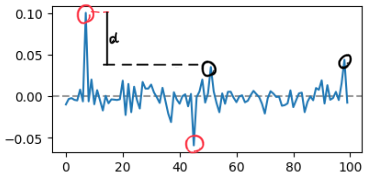
\includegraphics[scale = 0.7]{imgs/big_peaks.png}\\
        \captionof{figure}{}
    \end{center}
    As we can see the in (\textbf{Figure 1}) the 2 highest peaks are not very far from each other and that makes the order of magnitude lower compared to the peak we can see in the (\textbf{Figure 2}). Let's analyze two different meanings a peak can refer to:
    \begin{itemize}
        \item a strong movement in price
        \item a shock, due to news or particural events.
    \end{itemize}  
    Taking into consideration the nature of the sample taken, it is very unlikely to have two big shocks in the same window. Following this logic, when the $1^{st}$ and $2^{nd}$ peaks in a serie are close, we can conclude they are probably just strong movements in the price. Again, when the $1^{st}$ peak in terms of magnitude is way bigger than the $2^{nd}$, it is unlinkely to have price movements with this elevated magnitude, in very small ranges. We can note that since the usual price movement of these kind of stocks falls between a range of -0.01\% and 0.01\%, It seems reasonable to apply the scalar function to get an ultimate generated serie that can be used for data analysis purposes while reflecting the true nature of the financial asset. 
    \subsection*{Scalar Logic}
    Based on the above reasonment, the scalar assigns the value that usually shocks have in real data, to isolated peaks in the generated serie, adjusting it to a value plausible in real scenarios.
    It also assigns values typical of strong market movements, to peaks very close to each other.
    \subsection*{Scalar Implementation}
    The scalar computes the quantiles of the max values in the distribution and the same thing for the distribution of the difference between the $1^{st}$ and 
    $2^{nd}$ peaks.\\
    Then, the algorithm takes the sample to see where the distance between the $1^{st}$ and $2^{nd}$ peaks is, among the quantiles of the differences for real 
    data. A random value is then picked from a uniform distribution where the lower and upper bonudaries are the corresponding quantiles in the max distribution. 
    The same is applied to the negative peaks.
    \end{multicols}
    \textbf{Exemple:}
    \begin{center}
        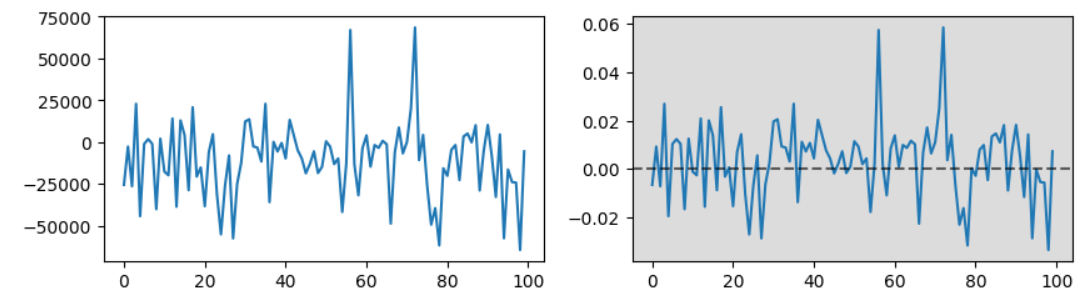
\includegraphics[scale=0.6]{imgs/EX_03.png}
    \end{center}
    In the above exemple we can see on the left, the serie generated by our model, and on the rigth the serie after the scaler is applied. As we can see,  
    the scaler preserves the pattern generated by our model and just rescales the data so that we have realistic data we can use for other experiments and implementations.



\begin{center}
    {\huge{Filter}}
\end{center}    
    \begin{multicols}{2}
    \section*{Problem}
    One problem we noticed in the samples generated by our model after the application of the filter is that some are really good and realistic, while others are 
    have no sense, for exemple let's take the samples shwon in the image below:
    \begin{center}
        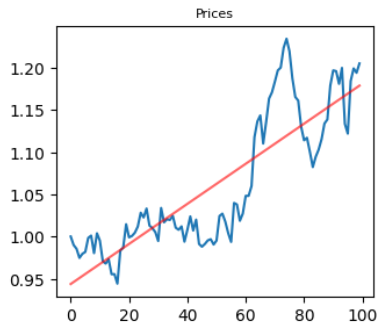
\includegraphics[scale=0.49]{imgs/serie_comp_1.png}
        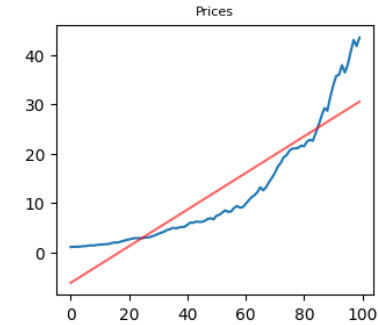
\includegraphics[scale=0.49]{imgs/serie_comp_2.png}
    \end{center}
    As we can see, the first series is very realistic while the other one is completly out of scale and shows a trend that is not 
    typical for fiancial time series. In order to solve this problem, we created a filter that selects from the samples generated the realistic series without modifyng the model output, so we end up with a realistic series dataset.
    \section*{How It works}
    To select the realistic series we came up with several metrics, the value of which can be tuned in the filter parameters:
    \paragraph*{Distance between residuals}
    We noticed that once we apply a linear regression to a series, the distance between consecutive residuals is smaller when the series shows an unrelistic behavior.
    In contrast, when we have a more realistic series the discance between consecutive points residuals is bigger.
    \begin{center}
        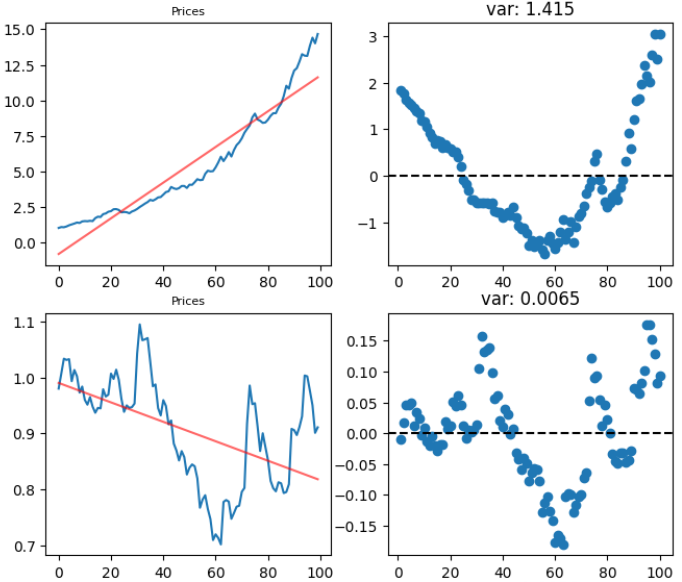
\includegraphics[scale=0.6]{imgs/2_res.png}
    \end{center}
    We scaled the price of the generated series between 0 and 1 to make it comparable and applied a linear regression to it. Once we obtained the linear regression, we computed the summation of the distance between consecutive residuals. 
    At this point, the filter just selects the series in which the summation of consecutive residuals is within a given threshold.\\
    \textbf{DfGenerator paramether}:  \textbf{variance\_th}.
    \paragraph*{Maximum range of oscillation}
    We decided to introcuce a parameter in the filter to chose the maximum range of oscillation between the first point an the last one in percentage. This is because we think it could be useful to have the freedom to decide the type of series we want 
    to generate to expand our dataset. Potentially we want to expand our dataset with very volatile series, in this case we can chose to use an hight max range of osscilation. Alternatively, our need could be to expand our dataset with more stable series, for example in order to decrease 
    the volatility of the predictions made by a model. In that case we can tune the parameter chosing a lower max range.\\
    \textbf{DfGenerator paramether}:  \textbf{max\_range}.

    \end{multicols}
    \newpage
    \begin{center}
        {\huge{Final Results}}
    \end{center} 
    The final result of the project is a program capable of generate realistic financial series such the following:
    \begin{center}
        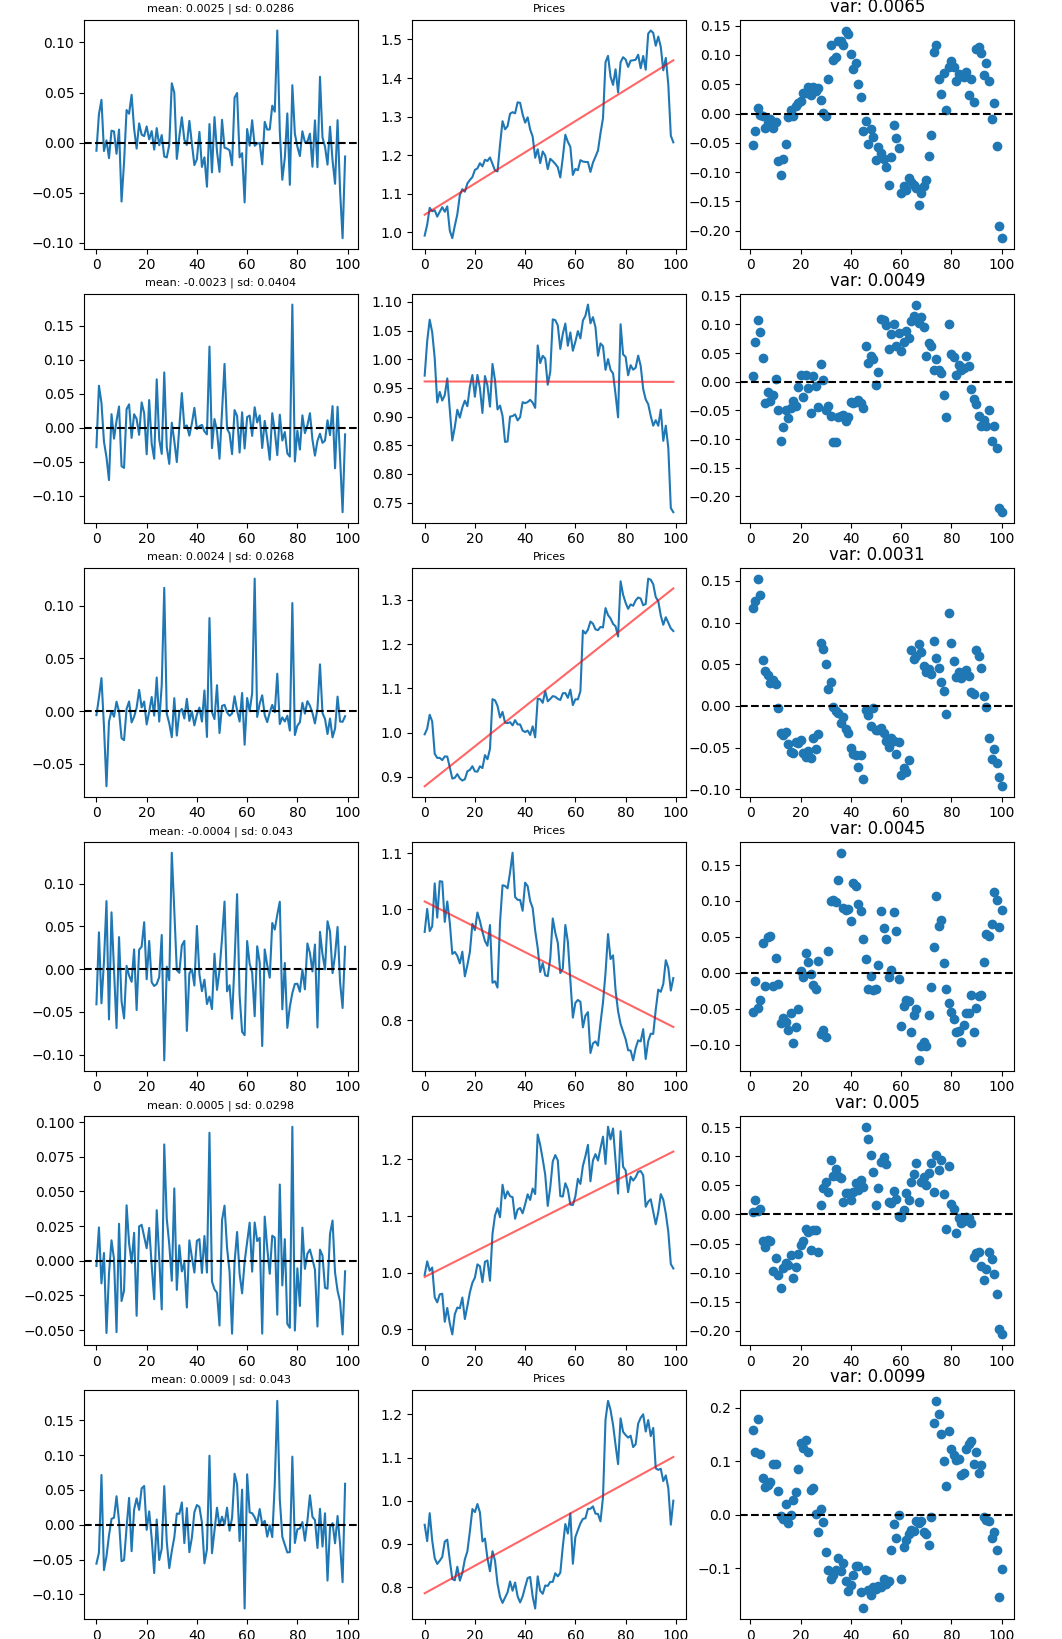
\includegraphics[scale=0.5]{imgs/results_reduced.png}
    \end{center}
    \newpage
    The generated series are visually similar to the original series. In the graph, the generated series are represented with a grey background to distinguish them from the original ones:
    \begin{center}
        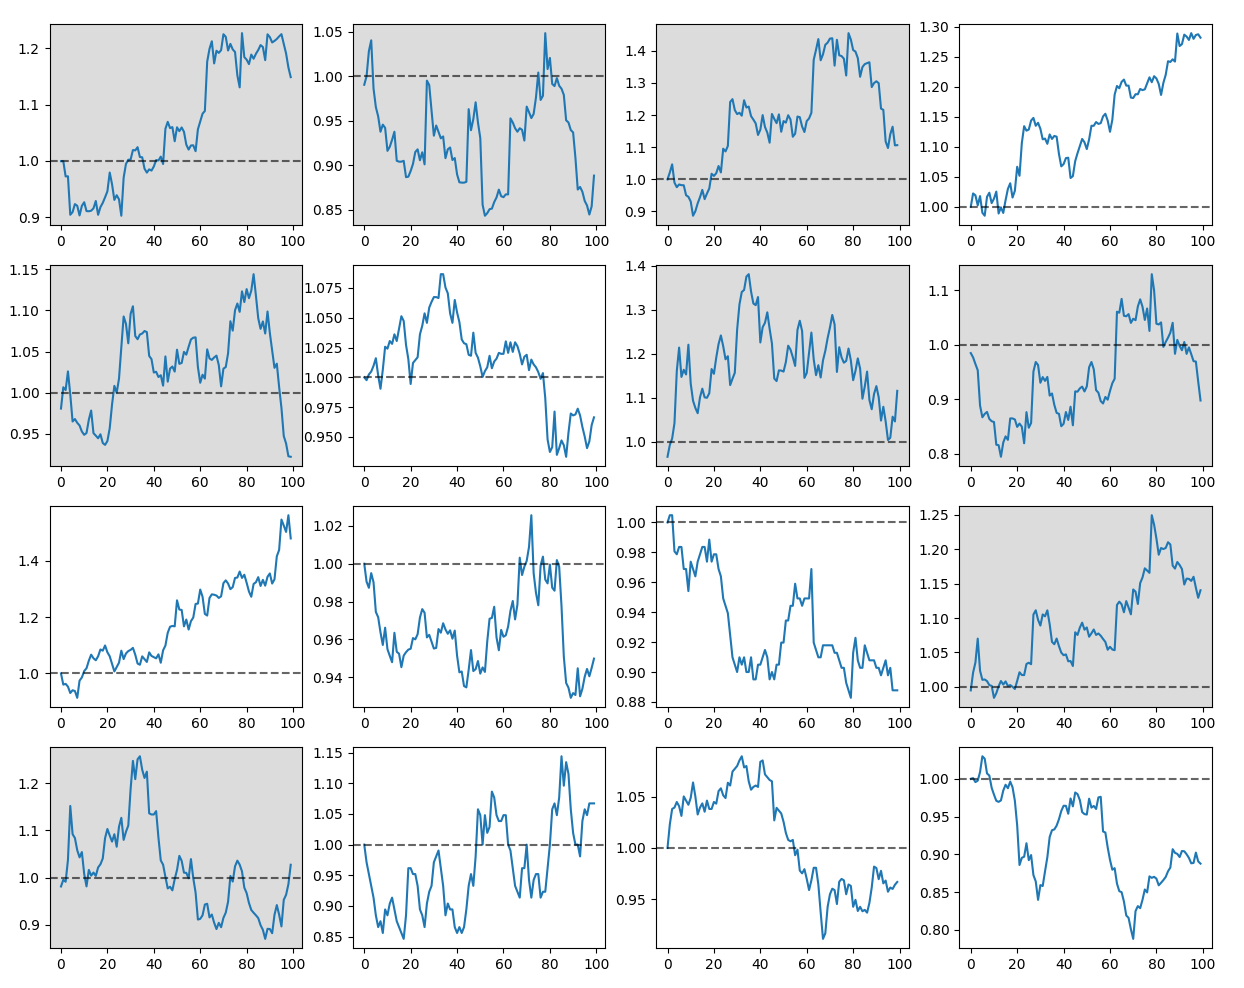
\includegraphics[scale=0.3]{imgs/series_comparison_README.png}
    \end{center}
    one of the main characteristic of retuns of financial series is the mean that is almost equal to 0. For that reason we tested if the mean of the returns generated by our model and the mean 
    of the real series of the dataset is the same. To do the following hypotesis test:
    \begin{equation}
        \begin{cases}
        H_0: \;\; \overline{X}=0\\
        H_1: \;\; \overline{X} \neq 0
    \end{cases}\,.
    \end{equation}
    $$T=\frac{\overline{X}-\mu_0}{S_n/\sqrt{n}} \;\;\;\;\;\;\;\;\;\;\; T|H_0 \sim t_{n-1}$$
    to test this hypothesis we generated a dataset of 10 000 samples an computed the mean: 0.00026567.
    The program takes approximatly 20 mintutes to generate a 10 000 samples dataset on a single cpu Intel Core I7. The distribution of the generated samples, looks like this:
    \begin{center}
        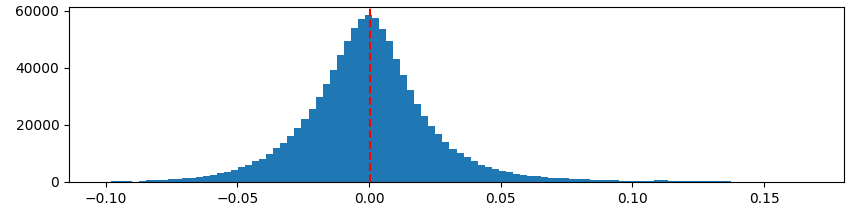
\includegraphics[scale=0.7]{imgs/generated.png}
    \end{center}
    
    \newpage
    \begin{center}
        {\huge{Future implementations}}
    \end{center} 
    here we want to briefly want to list some implementation we would like to work on in the Future:
    \begin{enumerate}
        \item Introduction of more rigorous mathematica text to test the realisticity of the series generated
        \item try more architectures
        \item implement a tensorboard interface to check models performance realtime during the training
        \item try to inlcude the rescaler in the model architecture of the generator so its paramethers can be optimized during the training
        \item try to feed the model with different types of dataset (e.g. specific sectors stocks) to see how this affect the results
        \item study the statistical properties of the series generated
        \item \textbf{expand a datataset and see how this affect the performances of a prediction model} 
    \end{enumerate}

    % \cite{Mindermann_2022}
    
    \begin{thebibliography}{9}
        \bibitem{Mindermann_2022}
        Mindermann, S., et al. (2022) \emph{Prioritized Training on Points that are learnable, Worth Learning, and Not Yet Learnt.}, \href{https://doi.org/10.48550/arXiv.2206.07137}{arXiv.2206.07.137}.
        
        \bibitem{}
        \end{thebibliography}

\end{document}
